
\subsection{Model Viewer Controller}
\begin{frame}
  \frametitle{Model Viewer Controller (MVC)}
  \framesubtitle{Idee}
  \begin{itemize}
    \item Sowohl Entwurfsmuster, also auch Designentwurf
    \item Hier Konzentration auf MVC-Architekturmuster
    \item Besteht aus drei Hauptkomponenten 
    \item Klare Trennung im Modell kann Aufwände verursachen (JavaFX) -> Siehe Beispiel
  \end{itemize}
\end{frame}

\begin{frame}
  \frametitle{Model Viewer Controller (MVC)}
  \framesubtitle{Struktur}
  \begin{figure}[ht]
    \centering
    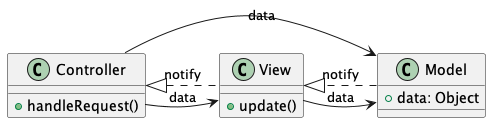
\includegraphics[width=0.7\textwidth]{fig/uml/default-mvc.png}
    \caption{Beispiel eines Basis MVC Architekturmusters}
    \label{fig:default-mvc}
  \end{figure}
\end{frame}

\begin{frame}
  \frametitle{Model Viewer Controller (MVC)}
  \framesubtitle{Fallbeispiel Led-Lampe}
  \begin{itemize}
    \item Mobile-App (Android Node) 
    \item Node.js Instanz (PI)
    \item Smarte Lampe  (Leuchtmittel mit ESP32) 
  \end{itemize}
\end{frame}

\begin{frame}
  \frametitle{Model Viewer Controller (MVC)}
  \framesubtitle{Struktur}
  \begin{figure}[ht]
    \centering
    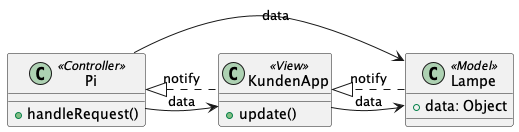
\includegraphics[width=0.7\textwidth]{fig/uml/sterotypen-mvc.png}
    \caption{MVC Architekturmusters im Fallbeispiel mit Sterotypen}
    \label{fig:stereo-mvc}
  \end{figure}
\end{frame}

\begin{frame}
  %\frametitle{Model Viewer Controller (MVC)}
  \framesubtitle{In Schichten: VCM und CVM}
  \begin{figure}[ht]
    \centering
    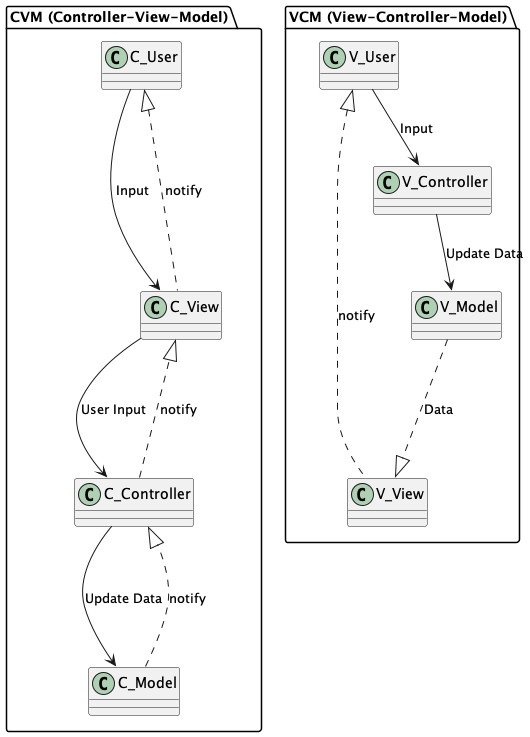
\includegraphics[width=0.40\textwidth]{fig/uml/mvc-varianten.png}
    \caption{Mögliche Varianten vom MVC in Schichten gedacht}
    \label{fig:mvs-varianten}
  \end{figure}
\end{frame}


\begin{frame}[fragile]
\begin{table}[ht]
\noindent\begin{minipage}[b]{1\linewidth}\centering
\begin{lstlisting}[caption={Java FX Input},captionpos=b,label={lst:javafx-input}]
public class JavaFXUserInputExample extends Application {

    public static void main(String[] args) {
        launch(args);
    }

    @Override
    public void start(Stage primaryStage) {
        Button button = new Button("Click me!");

        // Registering an EventHandler for the button click
        button.setOnAction(event -> {
            System.out.println("Button clicked!");
        });

        StackPane root = new StackPane();
        root.getChildren().add(button);

        Scene scene = new Scene(root, 300, 250);

        primaryStage.setTitle("JavaFX User Input Example");
        primaryStage.setScene(scene);
        primaryStage.show();
    }
}
\end{lstlisting}
\end{minipage}
\end{table}
\end{frame}

\subsection{Vertreter}
\begin{frame}
  \frametitle{Proxy}
  \framesubtitle{Idee}
  \begin{itemize}
    \item Zwischen Consumer und Provider platziert
    \item Ein Platzhalter, ein Vermittler
    \item Kann mit Caching Netzwerklatenz reduzieren
    \item Kann die Sicherheit erhöhen
  \end{itemize}
\end{frame}

\begin{frame}
  \frametitle{Proxy}
  \framesubtitle{Design als Pattern}
\begin{figure}[ht]
  \centering
  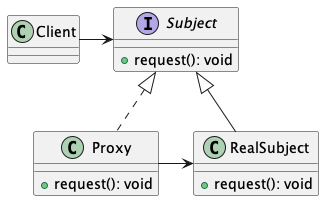
\includegraphics[width=0.45\textwidth]{fig/uml/proxy.png}
  \caption{Proxy Pattern}
  \label{fig:proxy}
\end{figure}
\end{frame}

\begin{frame}
  \frametitle{Proxy}
  \framesubtitle{Typen}
  \begin{itemize}
    \item Forward Proxy
    \item Reverse Proxy
    \item Caching Proxy
    \item Load Balancing Proxy
  \end{itemize}
\end{frame}

\begin{frame}
  \frametitle{Broker}
  \framesubtitle{Idee}
  \begin{itemize}
    \item Zwischen Consumer und Provider platziert
    \item Ein Vermittler mit erweiterten Funktionen
    \item Kann Nachrichten filtern, transformieren und aggregieren
    \item Unterstützt mehrere Protokolle
    \item Kann über eine Warteschlange für eine asynchrone Auslieferung verfügen
  \end{itemize}
\end{frame}

\begin{frame}
  \frametitle{Broker}
  \framesubtitle{Design als Pattern}
\begin{figure}[ht]
  \centering
  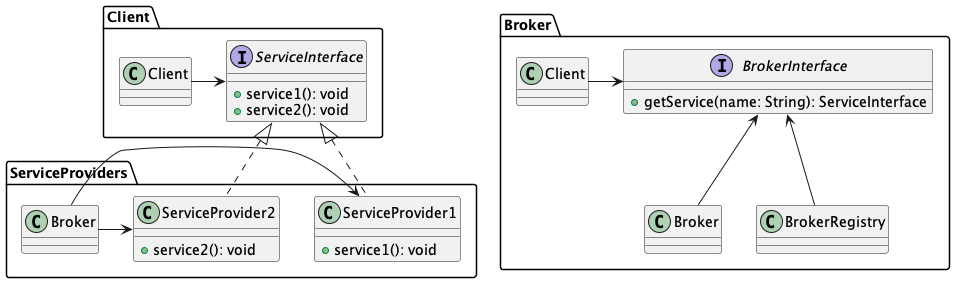
\includegraphics[width=1\textwidth]{fig/uml/broker.png}
  \caption{Broker Pattern}
  \label{fig:broker}
\end{figure}
\end{frame}

\begin{frame}
  \frametitle{Broker}
  \framesubtitle{Typen}
  \begin{itemize}
    \item Forwarding-Broker
    \item Handle-Driven-Broker 
  \end{itemize}
\end{frame}

\begin{frame}
  \frametitle{Trader}
  \framesubtitle{Idee}
  \begin{itemize}
    \item Zwischen Consumer und Provider platziert
    \item Ein Vermittler mit eigener Entscheidungskompetenz
    \item Kann Katalog von Diensten nach Kriterien anbieten
  \end{itemize}
\end{frame}